%-------------------------------------------------------------------------------
%                                PREAMBLE
%-------------------------------------------------------------------------------
\documentclass[usenames,dvipsnames,svgnames,10pt,aspectratio=169]{beamer}
%
\usefonttheme{professionalfonts}
% This theme uses TIKZ: compile twice with PDFLaTeX or LuaLaTeX.
%
%  Options:
%  - [clean]:    clean slides, i.e. logos and footbar are removed
%  - [kth]:      footbar style inspierd to the official KTH template
%  - [nicewave]: a different style of wave is used (not approved by FLOW)
%
\usetheme[kth]{flow}

\usepackage{hyperref,graphicx,lmodern}
\usepackage[utf8]{inputenc}
\usepackage{media9}
\usepackage{xcolor}
\usepackage{stmaryrd}
\usepackage{nicefrac}
\usepackage{multimedia}
\usepackage{multicol}
\usepackage{upgreek}
\usepackage[]{bm}
\usepackage[]{url}
\usepackage[]{animate}
\usepackage{amsmath}

\graphicspath{{imgs/}}
\setbeamertemplate{blocks}[rounded][shadow=true]


%-------------------------------------------------------------------------------
%                                TITLE PAGE
%-------------------------------------------------------------------------------
\title[Nonlinear physics] % Short title used in footline
{
	Nonlinear physics, dynamical \\
	systems and chaos theory
}

\author[J.-Ch.~Loiseau] % Presenting author in short form used in footline
{
	\underline{Jean-Christophe Loiseau}
}
% - Give the names in the same order as the appear in the paper.
% - Underline the presenting author.

\institute[unused]
{
	\url{jean-christophe.loiseau@ensam.eu} \\
	Laboratoire DynFluid \\
	Arts et M\'etiers, France.
}
% Keep it simple, no one is interested in your street address.

% University logo(s)
\logot{
\includegraphics[width=.128\paperwidth]{DynFluid_logo}}  % Top logo
\logob{
\includegraphics[width=0.128\paperwidth]{ENSAM_logo}} % Bottom logo
% \logoc[{\includegraphics[width=.128\paperwidth]{limsi}}]{\includegraphics[width=.128\paperwidth]{limsi}} % Corner logo
%
% Cover image: \cvrimg{x position}{y position}{cover image}
\cvrimg{.77}{.8}{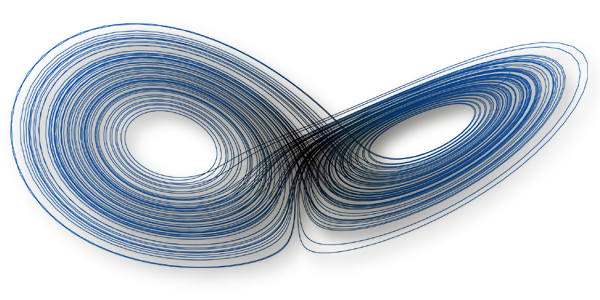
\includegraphics[width=.4\paperwidth]{cover.png}}

\date[unused]{Physique non-lin\'eaire -- 2019-2020}

\begin{document}

\titleframe	% Print the title as the first slide

%-------------------------------------------------------------------------------
%                           PRESENTATION SLIDES
%-------------------------------------------------------------------------------

\begin{frame}[t, c]{Basic information}{Organization}
	\begin{minipage}{.68\textwidth}
		\begin{itemize}
			\item Lectures will take place every Tuesdays and Thurdays, from 3:30pm to 5:30pm until late February.

			\bigskip

			\item Evaluation will be divided in two parts:
			\begin{itemize}
				\item[\( \hookrightarrow \)] A two-hour long written exam late February.
				\item[\( \hookrightarrow \)] A homework project involving mathematics and numerical simulations.
			\end{itemize}

			\medskip

			\item Do not hesitate to go through your linear algebra notes during Christmas vacation to refresh a bit!
		\end{itemize}
	\end{minipage}%
	\hfill
	\begin{minipage}{.28\textwidth}
		\centering
		
\includegraphics[width=\textwidth]{Gears}
	\end{minipage}

	\vspace{1cm}
\end{frame}

\begin{frame}[t, c]{Basic information}{Homework project}
	\begin{minipage}{.28\textwidth}
		\centering
		
\includegraphics[height=.15\textheight]{python_logo}

		\bigskip

		
\includegraphics[height=.15\textheight]{julia_logo}
	\end{minipage}%
	\hfill
	\begin{minipage}{.68\textwidth}
		\begin{itemize}
			\item Please use \alert{\textbf{Python 3}} or \alert{\textbf{Julia}}.
			\begin{itemize}
				\item[\( \hookrightarrow \)] Open-source programming languages with excellent scientific computing capabilities.
			\end{itemize}

			\medskip

			\item You can install both of them using \alert{\textbf{Anaconda}}.
			\begin{itemize}
				\item[\( \hookrightarrow \)] Available for Windows, Mac OS and Linux.
			\end{itemize}

			\medskip

			\item Numerous online resources to get familiar with both languages if needed, e.g.
			\begin{itemize}
				\item[\( \hookrightarrow \)] \url{https://www.codeacademy.com}
			\end{itemize}
		\end{itemize}
	\end{minipage}

	\vspace{1cm}
\end{frame}

\begin{frame}[t, c]{Basic information}{Useful references (in French)}
	\begin{minipage}{.58\textwidth}
		\begin{block}{\centering \textbf{General knowledge}}
			\begin{itemize}
				\item I.\ Stewart. \emph{Dieu joue-t'il au dés?} Flammarion (2004).

				\medskip

				\item J.\ Gleick. \emph{La théorie du chaos.} Flammarion (2008).

				\medskip

				\item I.\ Prigogine. \emph{Les lois du chaos.} Flammarion (2008).
			\end{itemize}
		\end{block}

		\medskip

		\begin{block}{\centering \textbf{Textbooks}}
			\begin{itemize}
				\item P.\ Bergé \emph{et al.} \emph{L'ordre dans le chaos.} Hermann (1998).

				\medskip

				\item P.\ Manneville. \emph{Instabilités, chaos et turbulence.} Ed.\ Ecole Polytechnique (2004).
			\end{itemize}
		\end{block}
	\end{minipage}%
	\hfill
	\begin{minipage}{.38\textwidth}
		\centering

		
\includegraphics[width=\textwidth]{references}
	\end{minipage}

	\vspace{1cm}
\end{frame}

% \begin{frame}[t, c]{Basic information}{Useful references (in English)}
% 	\begin{minipage}{.58\textwidth}
% 		\begin{block}{\centering \textbf{General knowledge}}
% 			\begin{itemize}
% 				\item I.\ Stewart. \emph{Dieu joue-t'il au dés?} Flammarion (2004).
%
% 				\medskip
%
% 				\item J.\ Gleick. \emph{La théorie du chaos.} Flammarion (2008).
%
% 				\medskip
%
% 				\item I.\ Prigogine. \emph{Les lois du chaos.} Flammarion (2008).
% 			\end{itemize}
% 		\end{block}
%
% 		\medskip
%
% 		\begin{block}{\centering \textbf{Textbooks}}
% 			\begin{itemize}
% 				\item P.\ Bergé \emph{et al.} \emph{L'ordre dans le chaos.} Hermann (1998).
%
% 				\medskip
%
% 				\item P.\ Manneville. \emph{Instabilités, chaos et turbulence.} Ed.\ Ecole Polytechnique (2004).
% 			\end{itemize}
% 		\end{block}
% 	\end{minipage}%
% 	\hfill
% 	\begin{minipage}{.38\textwidth}
% 		\centering
%
% 		
\includegraphics[width=\textwidth]{references}
% 	\end{minipage}
%
% 	\vspace{1cm}
% \end{frame}

%%%%%
%%%%%
%%%%%     Examples de systèmes dynamiques
%%%%%
%%%%%

\begin{frame}[t, c]{}{}
	\centering

	{\Large \textbf{What is a dynamical system?}}

	\bigskip

	\textgre{\textbf{A few examples}}

	\vspace{-2cm}
\end{frame}

\begin{frame}[t, c]{A few examples}{The double pendulum}
	\begin{minipage}{.28\textwidth}
		\centering
		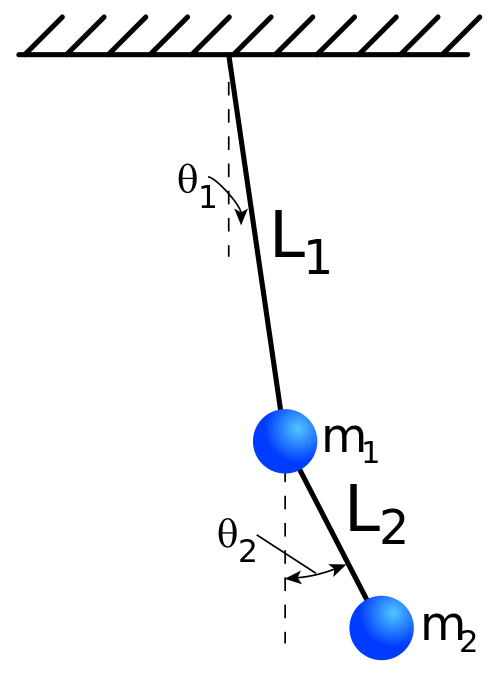
\includegraphics[width=.9\textwidth]{double_pendulum_geometry}
	\end{minipage}%
	\hfill
	\begin{minipage}{.68\textwidth}
		\begin{itemize}
			\item Its Lagrangian is
			%
			\begin{multline}
				\mathcal{L} = \overbrace{\frac{1}{2} m_1 l_1^2 \dot{\theta}_1^2 + \frac{1}{2} m_2 \left( l_1^2 \dot{\theta}_1^2 + l_2^2 \dot{\theta}_2^2 + 2 l_1 l_2 \dot{\theta}_1 \dot{\theta}_2 \cos \left( \theta_1 - \theta_2 \right) \right)}^{\textrm{Kinetic energy}} \\
				\underbrace{- (m_1 + m_2) g l_1 \cos \theta_1 - m_2 g l_2 \cos \theta_2}_{\textrm{Potential energy}}.
				\notag
			\end{multline}

			\item Equations of motions are given by
			%
			\[
				\frac{\mathrm{d}}{\mathrm{d}t} \left(	\frac{\partial \mathcal{L}}{\partial \dot{\theta}_i} \right) - \frac{\partial \mathcal{L}}{\partial \theta_i} = 0.
			\]

			\item Nonlinear system of ODEs.
			\begin{itemize}
				\item[\( \hookrightarrow \)] Very few analytical solutions are known.
			\end{itemize}
		\end{itemize}
	\end{minipage}

	\vspace{1cm}
\end{frame}

\begin{frame}[t, c]{A few examples}{The double pendulum}
	\begin{minipage}{.48\textwidth}
		\begin{itemize}
			\item Simple mechanical sytem exhibiting nonetheless complex dynamics.

			\bigskip

			\item Evolutions of similar initial conditions diverge exponentially fast.
			\begin{itemize}
				\item[\( \hookrightarrow	\)] Hallmark of chaotic dynamics.
			\end{itemize}

			\medskip

			\item Limited prediction horizon despite its deterministic equations of motion.
		\end{itemize}
	\end{minipage}%
	\hfill
	\begin{minipage}{.48\textwidth}
		\vspace{-1cm}
		\begin{center}
			\movie[width=\textwidth, autostart, loop]{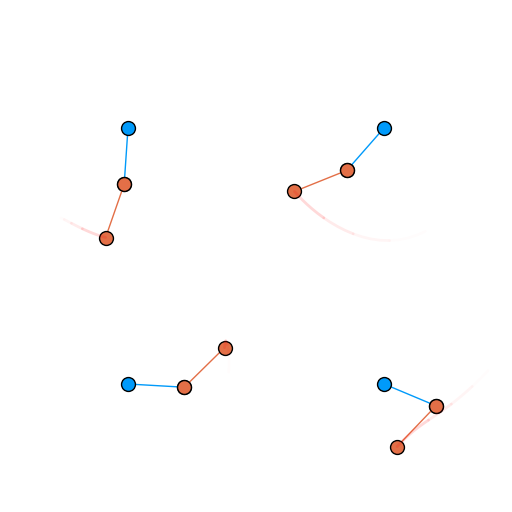
\includegraphics[width=\textwidth]{double_pendulum}}{imgs/double_pendulum.mp4}
		\end{center}
	\end{minipage}

	\vspace{1cm}
\end{frame}

\begin{frame}[t, c]{A few examples}{Prey-Predator system}
	\begin{minipage}{.48\textwidth}
		\centering
		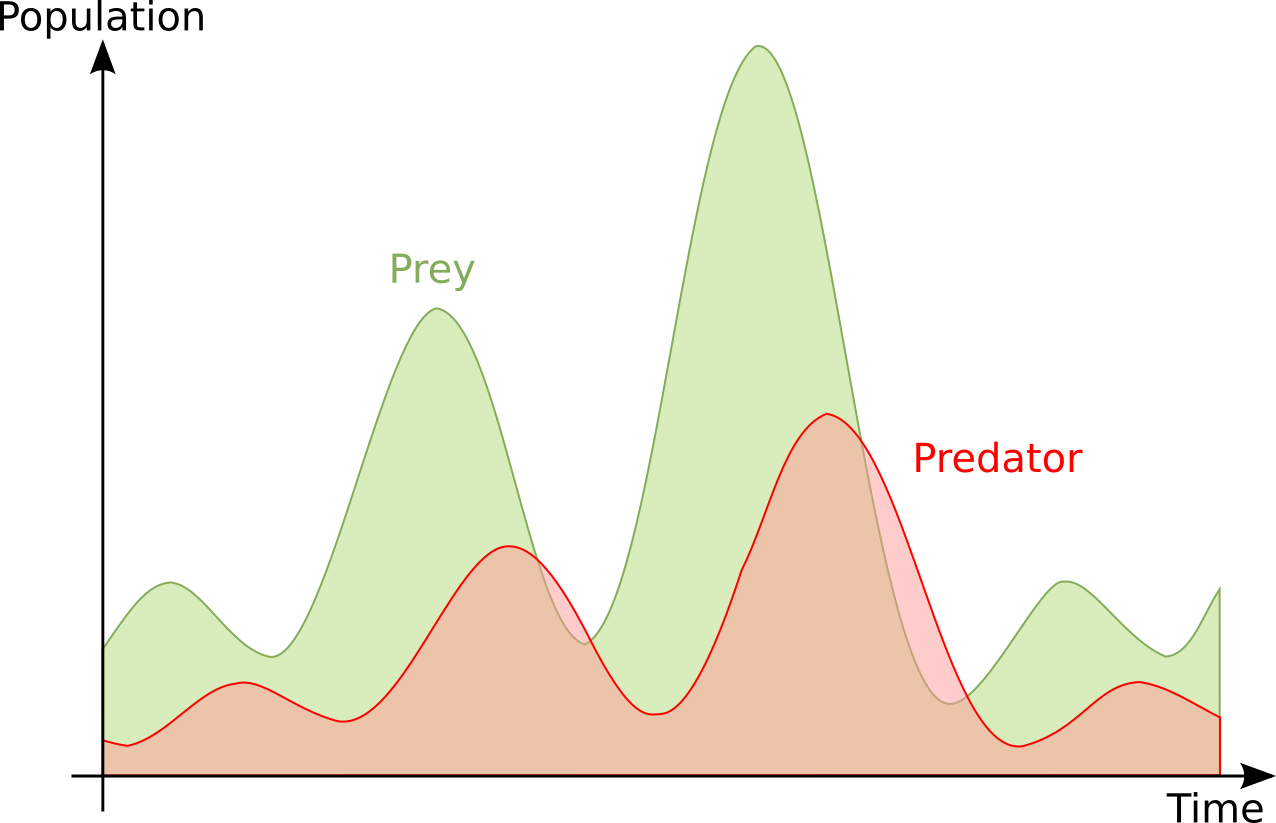
\includegraphics[width=\textwidth]{Lotka_Volterra}
	\end{minipage}%
	\hfill
	\begin{minipage}{.48\textwidth}
		\begin{itemize}
			\item Dynamics of a prey-predator system can be modeled as
			%
			\[
				\begin{aligned}
					\frac{\mathrm{d}x}{\mathrm{d}t} & = \alpha x - \beta xy \\
					\frac{\mathrm{d}y}{\mathrm{d}t} & = - \gamma y + \delta xy.
				\end{aligned}
			\]
			\medskip

			\item Describes the observations of hares and lynx populations in Canada in the early 1900's.
		\end{itemize}
	\end{minipage}

	\vspace{1cm}
\end{frame}

\begin{frame}[t, c]{A few examples}{Chemical reaction-diffusion systems}
	\begin{minipage}{.38\textwidth}
		\centering
		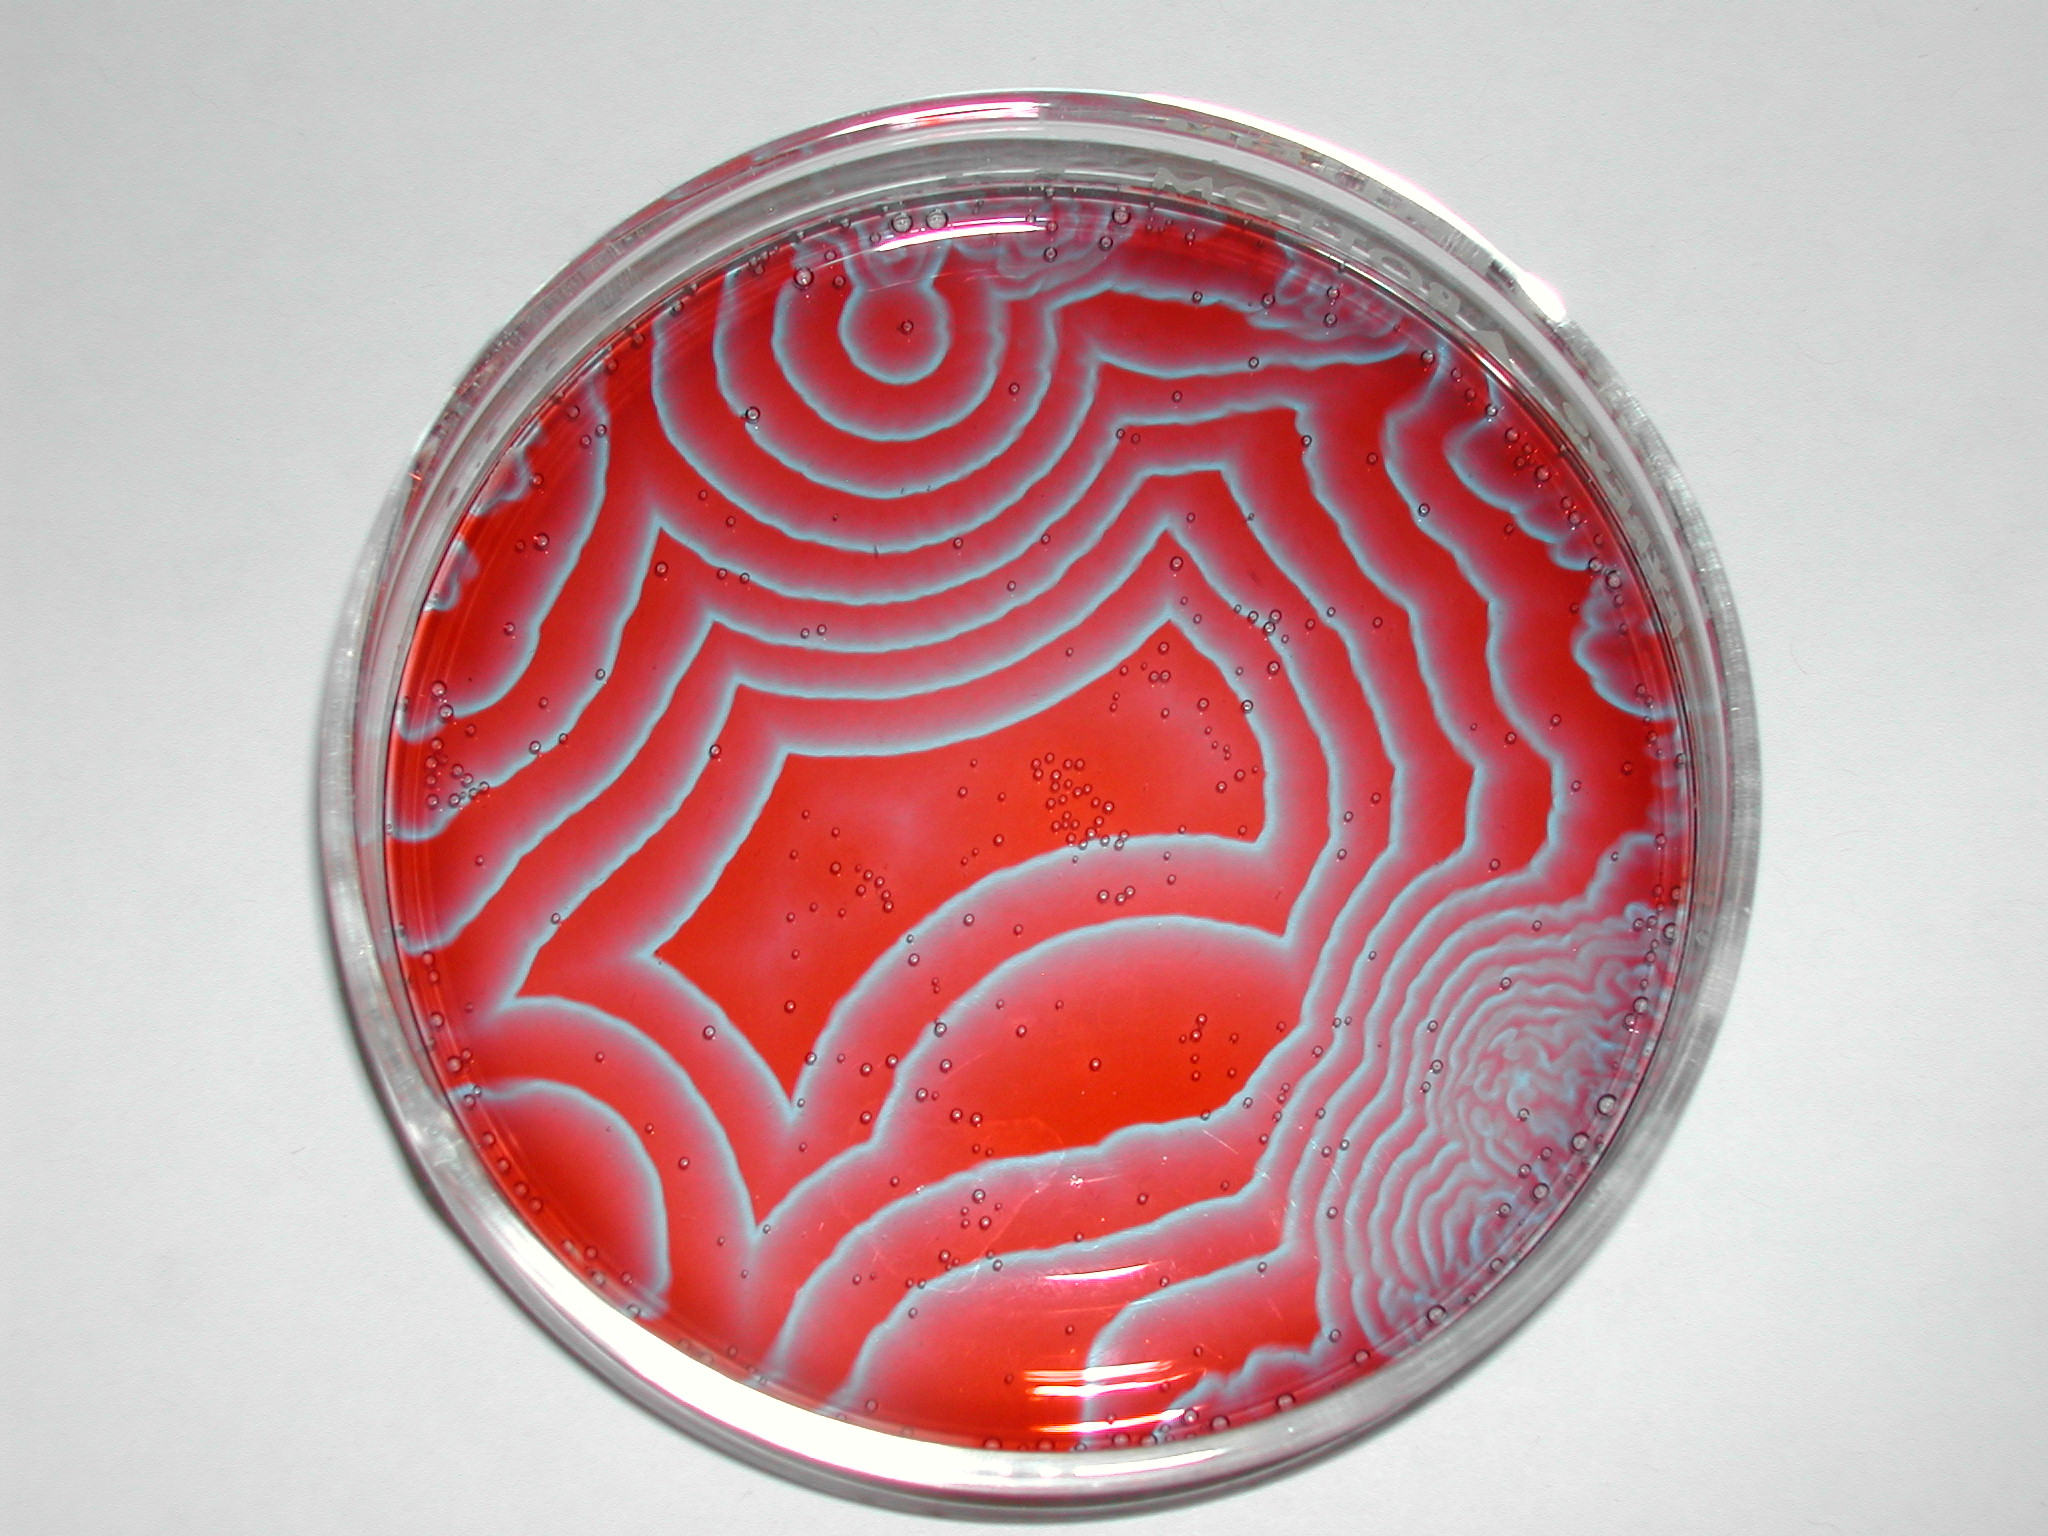
\includegraphics[width=\textwidth]{BZ_reaction}
	\end{minipage}%
	\hfill
	\begin{minipage}{.58\textwidth}
		\begin{itemize}
			\item Spatio-temporal reaction-diffusion systems can be modeled as
			%
			\[
				\frac{\partial \bm{q}}{\partial t} = \bm{D} \nabla^2 \bm{q} + \mathcal{R}(\bm{q}),
			\]
			%
			where \(\bm{D}\) describes the diffusion of each species and \( \bm{R}(\bm{q}) \) the inter-species reactions.

			\bigskip

			\item Set of nonlinear partial differential equations exhibiting suprising physical phenomena!
			\begin{itemize}
				\item[\( \hookrightarrow \)] Traveling waves, pattern formation, spatiotemporal chaos, etc.
			\end{itemize}
		\end{itemize}
	\end{minipage}

	\vspace{1cm}
\end{frame}

\begin{frame}[t, c]{A few examples}{Incompressible flow past cylinders}
	\begin{minipage}{.48\textwidth}
		\begin{itemize}
			\item Dynamics are governed by the Navier-Stokes equations
			%
			\[
				\begin{aligned}
					\displaystyle \frac{\partial {\bm u}}{\partial t} + ({\bm u} \cdot \nabla ) {\bm u} & = - \nabla p + \frac{1}{Re}\nabla^2 {\bm u} + {\bm f}\\
					\nabla \cdot {\bm u} & = 0.
				\end{aligned}
			\]

			\medskip

			\item Set of nonlinear partial differential equations.

			\bigskip

			\item Give rise to an extremely high-dimensional nonlinear system once discretized!
			\begin{itemize}
				\item[\( \hookrightarrow \)] 10\textsuperscript{5} to 10\textsuperscript{10} degrees of freedom.
			\end{itemize}
		\end{itemize}
	\end{minipage}%
	\hfill
	\begin{minipage}{.48\textwidth}
		\begin{center}
			\movie[width=\textwidth, autostart, loop]{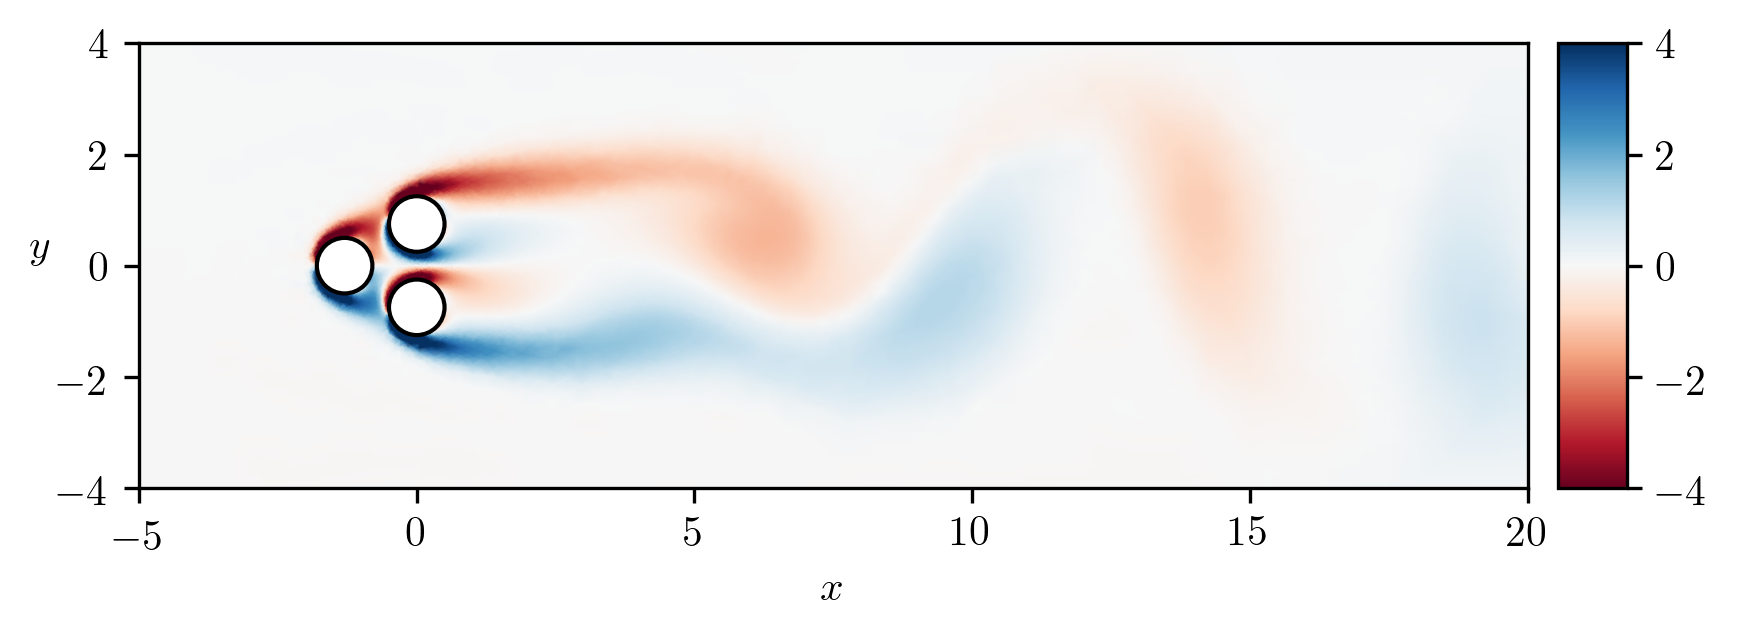
\includegraphics[width=\textwidth]{fluidic_pinball_Re60_snapshot}}{imgs/fluidic_pinball_Re60.mp4}
		\end{center}
	\end{minipage}

	\vspace{1cm}
\end{frame}

% \begin{frame}[t, c]{Quelques exemples...}{L'écoulement autour d'un cylindre}
% 	\begin{minipage}{0.48\textwidth}
% 		\begin{itemize}
% 			\item La dynamique de l'écoulement est gouvernée par les équations de Navier-Stokes
% 			\begin{equation}
% 				\begin{aligned}
% 					\displaystyle \frac{\partial {\bm u}}{\partial t} + ({\bm u} \cdot \nabla ) {\bm u} & = - \nabla p + \frac{1}{Re}\nabla^2 {\bm u} + {\bm f}\\
% 					\nabla \cdot {\bm u} & = 0.
% 				\end{aligned}
% 				\notag
% 			\end{equation}
%
% 			\item Ce sont des équations non-linéaires aux dérivées partielles.
% 			\begin{itemize}
% 				\item[$\hookrightarrow$] Très peu de solutions analytiques.
% 			\end{itemize}
%
% 		\end{itemize}
% 	\end{minipage}%
% 	\hfill
% 	\begin{minipage}{0.48\textwidth}
% 		\begin{center}
% 			\movie[width=\textwidth, autostart, loop]{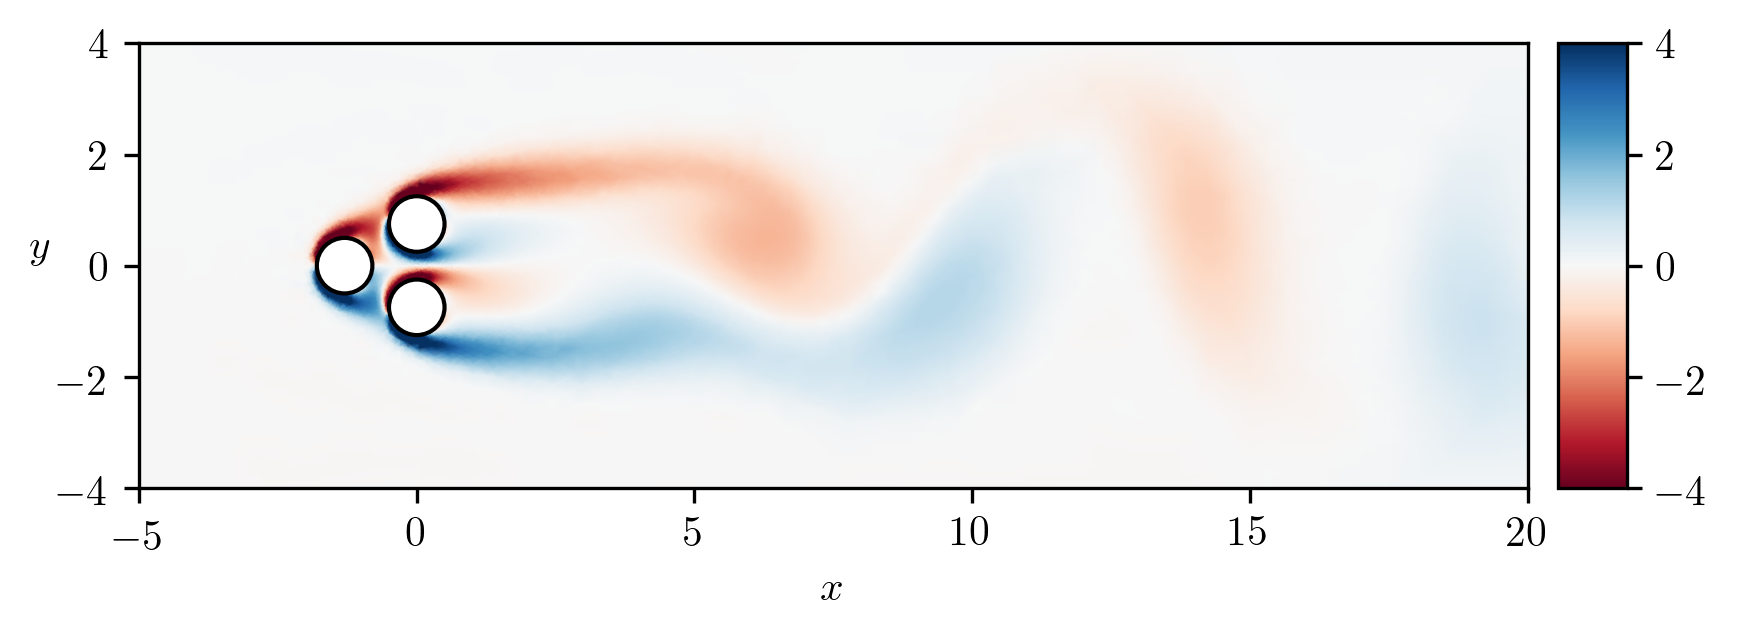
\includegraphics[width=\textwidth]{fluidic_pinball_Re60_snapshot}}{imgs/fluidic_pinball_Re60.mp4}
% 		\end{center}
%
% 		{\small Evolution temporelle du champ de vorticité autour d'un trio de cylindre. Notez que la vitesse de rotation des cylindres n'est pas constante.}
% 	\end{minipage}
% \end{frame}


% \begin{frame}[t, c]{Quelques exemples...}{Systèmes dynamiques en temps continu}
%
% 	\begin{itemize}
% 		\item Tous ces systèmes peuvent être écrits sous la forme
% 		\begin{equation}
% 			\dot{\bm x} = \bm{f}({\bm x}, \lambda)
% 			\notag
% 		\end{equation}
% 		où ${\bm x}$ est le \emph{vecteur d'état} du système, $\lambda$ un vecteur de \emph{paramètres} et $\bm{f}({\bm x}, \lambda)$ une fonction non-linéaire.
%
% 		\bigskip
%
% 		\item \`A noter que l'on pré-suppose ici que le temps $t$ est continu.
% 	\end{itemize}
%
% 	\vspace{1cm}
% \end{frame}
%
% \begin{frame}[t, c]{Quelques exemples...}{Systèmes dynamiques en temps discret}
%
% 	\begin{itemize}
% 		\item Si l'on a qu'une vue \emph{stroboscopique} du système, sa dynamique peut alors être exprimée de la façon suivante
% 		\begin{equation}
% 			{\bm x}^{(n+1)} = \bm{F}({\bm x}^{(n)}, \lambda)
% 			\notag
% 		\end{equation}
% 		où $n$ définie maintenant l'instant discret.
%
% 		\bigskip
%
% 		\item Ce genre de modèle est appelé un \emph{système dynamique à temps discret}, un \emph{itéré} ou encore une \emph{map}.
% 	\end{itemize}
%
% 		\vspace{1cm}
% \end{frame}


%%%%%
%%%%%
%%%%%     Quelques définitions nécessaires pour la suite
%%%%%
%%%%%

\begin{frame}[t, c]{}{}
		\centering

		{\Large \textbf{How do we study dynamical systems?}}

		\bigskip

		\textgre{\textbf{A quick overview of what's coming.}}

		\vspace{-2cm}
\end{frame}

\begin{frame}[t, c]{How do we study dynamical systems?}{Mathematical frameworks}
	\begin{minipage}{.48\textwidth}
		\begin{itemize}
			\item All of the examples considered are governed by equations of the form
			%
			\[
				\frac{\mathrm{d}\bm{x}}{\mathrm{d}t} = \bm{f}\left(	\bm{x}, \boldsymbol{\mu} \right),
			\]
			%
			with \(\bm{x}\) the state vector and \(\boldsymbol{\mu}\) the vector of parameters.

			\medskip

			\item In general, the function \( \bm{f}\left( \bm{x}, \boldsymbol{\mu} \right)\) is a \emph{nonlinear} function of the state.

			\medskip

			\item Skimming through your lecture notes on \emph{ordinary differential equations} might be a good idea.
		\end{itemize}
	\end{minipage}%
	\hfill
	\begin{minipage}{.48\textwidth}
		\centering
		
\includegraphics[width=\textwidth]{still_waiting}
	\end{minipage}

	\vspace{1cm}
\end{frame}

\begin{frame}[t, c]{What is a linear system?}{}
	\centering

	\begin{block}{}
		\centering
		Let us consider the following system
		%
		\[
			\dot{\bm x} = {\bm f}({\bm x}).
		\]
		%
		Under which condition(s) is it \alert{\textbf{linear}}?
	\end{block}

	\vspace{1cm}
\end{frame}

\begin{frame}[t, c]{What is a linear system?}{A few definitions}
	\begin{itemize}
		\item Consider \(\bm{u}(t)\) and \(\bm{v}(t)\) two solutions of our system.

		\medskip

		\item A system is said to be \alert{\textbf{linear}} if:
		\begin{itemize}
			\item[\( \hookrightarrow \)] \(\bm{w}(t) = \alpha \bm{u}(t) + \beta \bm{v}(t) \) is also solution,
			\item[\( \hookrightarrow \)] \(\bm{f}\left(	\alpha \bm{u} + \beta \bm{v} \right) = \alpha \bm{f}(\bm{u}) + \beta \bm{f}(\bm{v}) \),
			\item[\( \hookrightarrow \)] It satisfies the \alert{\textbf{superposition principle}}.
		\end{itemize}

		\item If so, it can be rewritten as
		%
		\[
			\frac{\mathrm{d}\bm{x}}{\mathrm{d}t} = \bm{Ax},
		\]
		%
		where \( \bm{A} \) is a linear operator (i.e.\ a matrix).

		\medskip

		\item The general solution is given by
		%
		\[
			\bm{x}(t) = e^{\bm{A}t} \bm{x}_0.
		\]
	\end{itemize}
	\vspace{1cm}
\end{frame}

\begin{frame}[t, c]{What is a linear system?}{Example: the harmonic oscillator}
	\begin{minipage}{.38\textwidth}
		\centering
		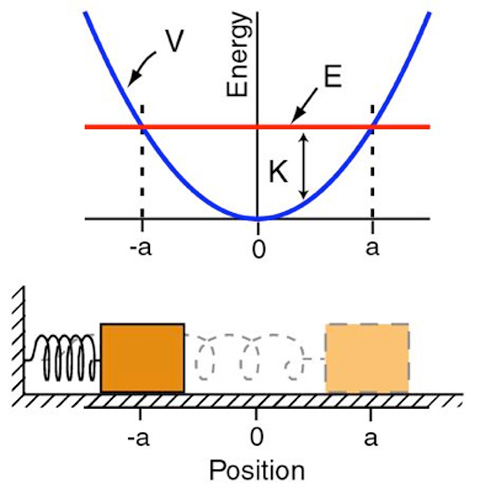
\includegraphics[width=.8\textwidth]{harmonic_oscillator}
	\end{minipage}%
	\hfill
	\begin{minipage}{.58\textwidth}
		\begin{itemize}
			\item Dynamics of a (damped) harmonic oscillator are governed by
			%
			\[
				\ddot{x} = -2k \dot{x} - \omega_0^2 x.
			\]

			\medskip

			\item Introducing \( y = \dot{x} \), we can recast it as
			%
			\[
				\displaystyle \frac{\mathrm{d}}{\mathrm{d}t} \begin{bmatrix} x \\ y \end{bmatrix} = \begin{bmatrix} 0 & 1 \\ -\omega_0^2 & -2k \end{bmatrix} \begin{bmatrix} x \\ y \end{bmatrix}.
			\]

			\medskip

			\item Depending on the friction parameter \(k\), the system can be overdamped, under-damped or criticaly damped.
			\begin{itemize}
				\item[\( \hookrightarrow \)] Each regime corresponds to different dynamics.
			\end{itemize}
		\end{itemize}
	\end{minipage}

	\vspace{1cm}
\end{frame}

\begin{frame}[t, c]{What is alinear system?}{Example: the harmonic oscillator}
	\centering
	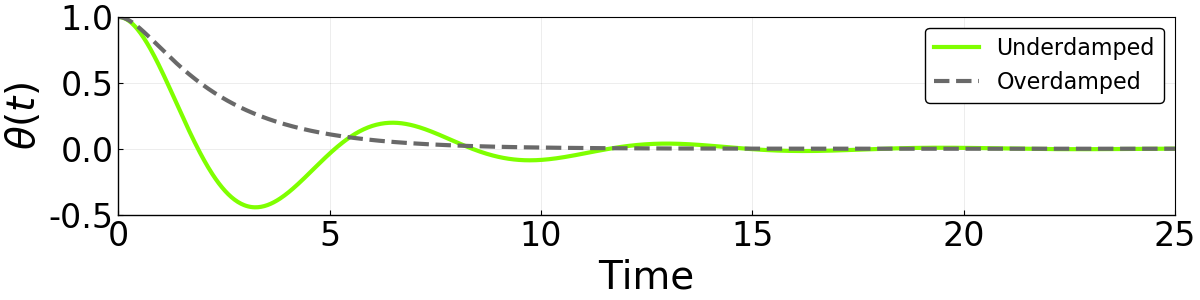
\includegraphics[width=.9\textwidth]{harmonic_oscillator_regimes}
	\vspace{1cm}
\end{frame}

\begin{frame}[t, c]{What is a linear system?}{Example: the Orr-Sommerfeld-Squire equations}
	\begin{minipage}{.58\textwidth}
		\begin{itemize}
			\item OSS equations are a reformulation of the linearized Navier-Stokes equations.
			\begin{itemize}
				\item[\( \hookrightarrow \)] See your hydrodynamic instability class for more details.
			\end{itemize}

			\medskip

			\item In matrix form, they read
			%
			\[
				\displaystyle \frac{\mathrm{d}}{\mathrm{d}t} \begin{bmatrix} \bm{v} \\ \bm{\eta} \end{bmatrix} = \underbrace{\begin{bmatrix} \bm{L}_{OS} & 0 \\ \bm{C} & \bm{L}_S \end{bmatrix}}_{\mathcal{L}} \begin{bmatrix} \bm{v} \\ \bm{\eta} \end{bmatrix},
			\]
			%
			with \(\bm{v}\) the wall normal velocity and \(\bm{\eta}\)\\ the vorticity.

			\medskip

			\item Describe the evolution of infinitesimal \\ perturbations in parallel shear flows.
		\end{itemize}
	\end{minipage}%
	\hfill
	\begin{minipage}{.38\textwidth}
		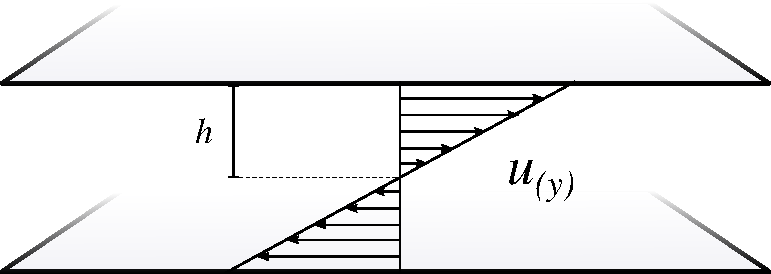
\includegraphics[width=\textwidth]{Couette_flow}

		\bigskip

		\hspace{-2.5cm} 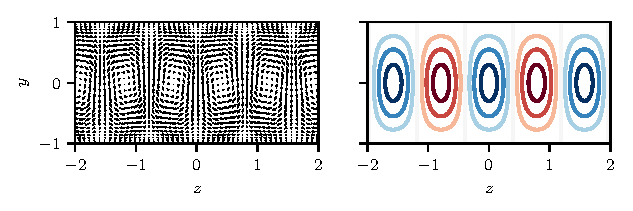
\includegraphics[width=1.5\textwidth]{S2_optimal_perturbation_couette_flow}
	\end{minipage}

	\vspace{1cm}
\end{frame}

\begin{frame}[t, c]{}{}
	\begin{block}{\centering \textbf{Warning!}}
		If linear systems have appeared so frequently during the course of your studies, it is solely because they are easy to study!
		Most linear systems are actually only an approximation of a more complex (but more realistic) nonlinear system.
	\end{block}
\end{frame}

\begin{frame}[t, c]{What is a nonlinear system?}{}
	\centering

	\begin{block}{}
		\centering
		Let us consider the following system
		%
		\[
			\dot{\bm x} = {\bm f}({\bm x}).
		\]
		%
		Under which condition(s) is it \alert{\textbf{nonlinear}}?
	\end{block}

	\vspace{1cm}
\end{frame}

\begin{frame}[t, c]{What is a nonlinear system?}{Example: photon emission in laser}
	\begin{minipage}{.58\textwidth}
		\begin{itemize}
			\item Photon emission in a laser can be modeled by
			%
			\[
				\dot{n} = gn(N_0 - an) - kn
			\]
			%
			where \(g\) is the gain of the laser, \(k\) describe the loss and \(N(t) = N_0 - an\) is the number of excited atoms.

			\medskip

			\item It can be recast as
			%
			\[
				\dot{x} = \mu x - x^2.
			\]

			\item It is a first-order nonlinear ordinary differential equations.

			\medskip

			\item We do not have a closed-form solution despite the apparent simplicity of the equation.

		\end{itemize}
	\end{minipage}%
	\hfill
	\begin{minipage}{.38\textwidth}
		\hspace{-0.75cm} 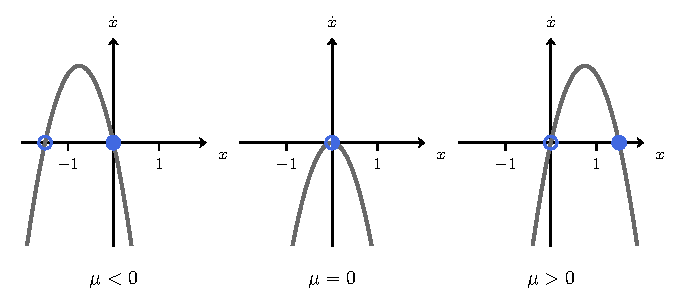
\includegraphics[width=1.2\textwidth]{transcritical_phase_line}
	\end{minipage}

	\vspace{1cm}
\end{frame}

\begin{frame}[t, c]{What is a nonlinear system?}{Example: the van der Pol oscillator}
	\begin{minipage}{.38\textwidth}
		\centering
		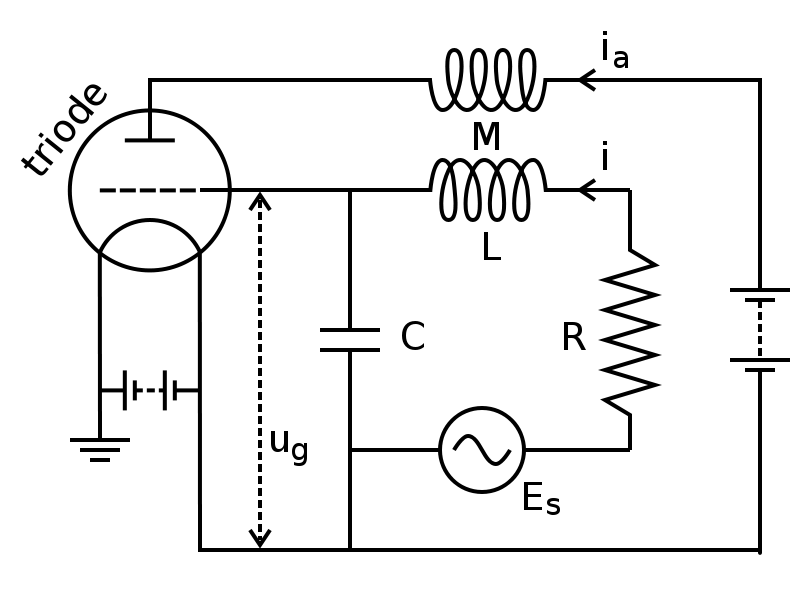
\includegraphics[width=\textwidth]{van_der_pol}
	\end{minipage}%
	\hfill
	\begin{minipage}{.58\textwidth}
		\begin{itemize}
			\item The equations governing this eletrical circuit are
			%
			\[
				\ddot{x} - \mu (1 - x^2) \dot{x} + x = 0.
			\]

			\medskip

			\item It is known as the \emph{Van der Pol oscillator}.
			\begin{itemize}
				\item[\( \hookrightarrow	\)] It is a non-conservative oscillator with nonlinear damping.
			\end{itemize}

			\bigskip

			\item It serves to model a large variety of physical systems.
			\begin{itemize}
				\item[\( \hookrightarrow \)] Action potentials of neurons, interaction between two plates in a geological fault, \ldots
			\end{itemize}
		\end{itemize}
	\end{minipage}

	\vspace{1cm}
\end{frame}

\begin{frame}[t, c]{What is a nonlinear system?}{Example: the van der Pol oscillator}
	\begin{minipage}{.58\textwidth}
		\begin{itemize}
			\item Standard model to study the properties of simple nonlinear oscillators.

			\bigskip

			\item The shape of the \emph{limit cycle} in the \((x, \dot{x})\) plane varies drastically as \(\mu\) increases.

			\bigskip

			\item When forcing the system at certain frequencies, the dynamics become chaotic.
		\end{itemize}
	\end{minipage}%
	\hfill
	\begin{minipage}{.38\textwidth}
		\centering
		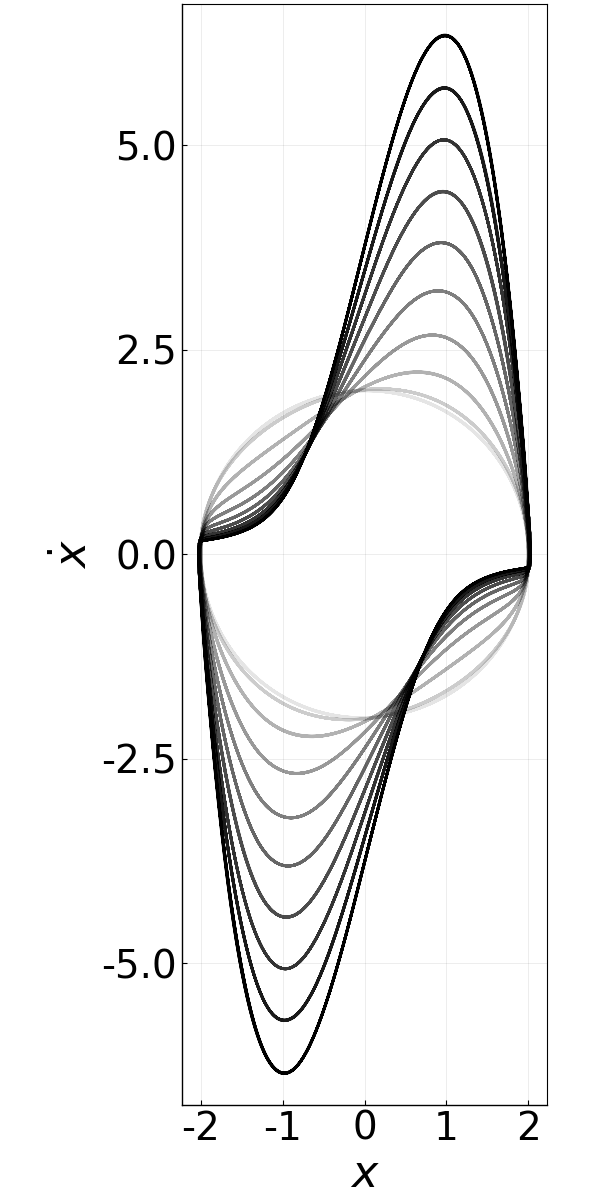
\includegraphics[height=.75\textheight]{van_der_pol_limit_cycle}
	\end{minipage}

	\vspace{1cm}
\end{frame}

\begin{frame}[t, c]{}{}
	\centering

	{\Large \textbf{Case study I}}

	\bigskip

	\textgre{\textbf{The simple pendulum}}

	\vspace{-2cm}
\end{frame}

\begin{frame}[t, c]{The simple pendulum}{Governing equations}
	\begin{minipage}{.68\textwidth}
		\begin{itemize}
			\item The governing equations read
			%
			\[
				\ddot{\theta} + 2k \dot{\theta} + \omega_0^2 \sin(\theta) = 0,
			\]
			%
			with \( k \) the friction coefficient and \( \omega_0^2 = \nicefrac{g}{L} \) the natural frequency of the pendulum.

			\bigskip

			\item Introducing \( x = \theta \) and \( y = \dot{\theta} \), we can recast it as a system of first-order ODEs
			%
			\[
				\begin{aligned}
					& \dot{x} = y \\
					& \dot{y} = -2k y - \omega_0^2 \sin(x).
				\end{aligned}
			\]

			\medskip

			\item Let's study in details the properties of this dynamical system.
		\end{itemize}
	\end{minipage}%
	\hfill
	\begin{minipage}{.28\textwidth}
		\centering
		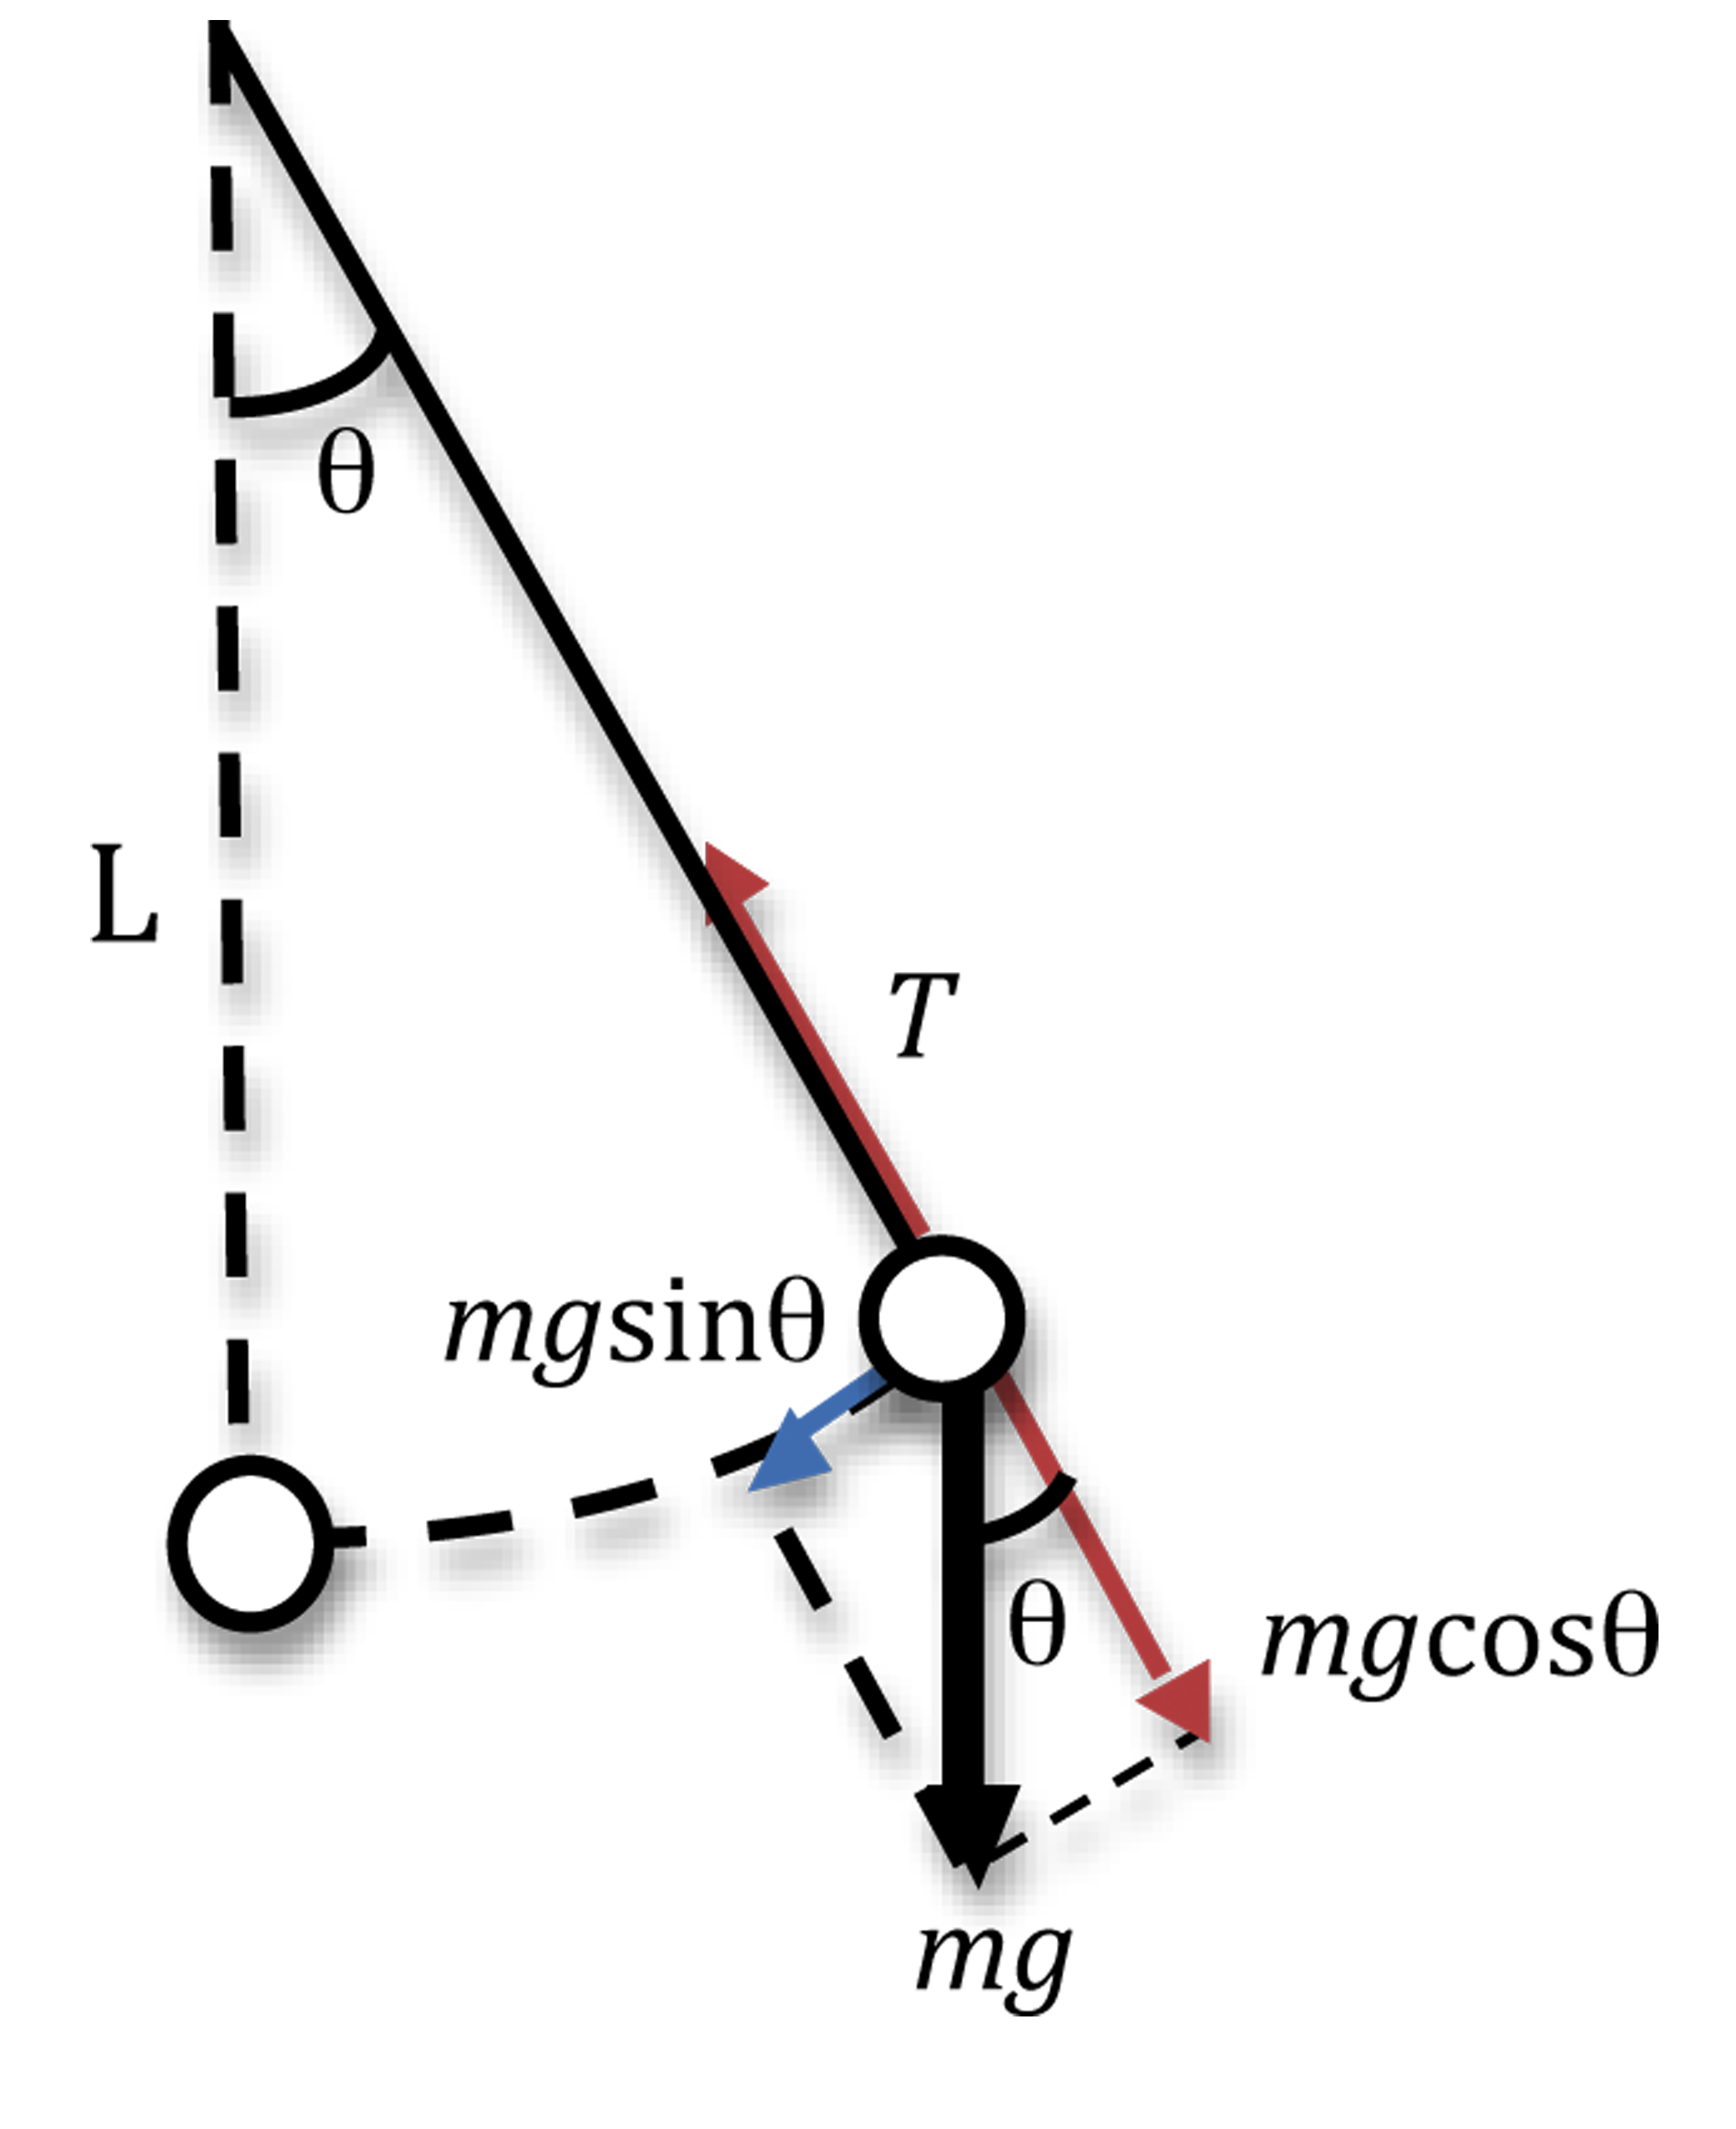
\includegraphics[width=\textwidth]{pendulum_sketch}
	\end{minipage}

	\vspace{1cm}
\end{frame}

\begin{frame}[t, c]{The simple pendulum}{Phase plane representation}
	\centering
	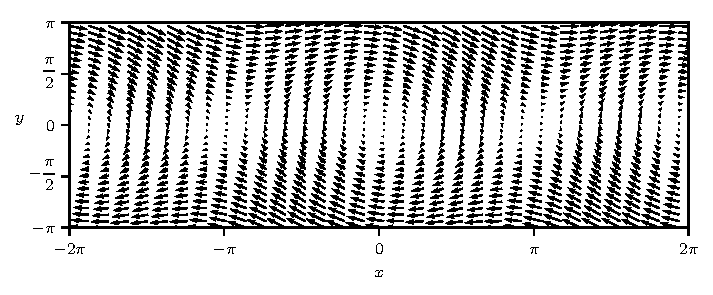
\includegraphics[width=.8\textwidth]{pendulum_phase_plane}
\end{frame}

\begin{frame}[t, c]{The simple pendulum}{Fixed points}
	\begin{minipage}{.68\textwidth}
		\begin{itemize}
			\item There are a few points of the phase plane where the system is in equilibrium.
			These are known as \alert{\textbf{fixed points}}.
			They satisfy the equations
			%
			\[
				\dot{x} = 0 \text{ and } \dot{y} = 0.
			\]

			\item For the simple pendulum, these fixed points are solution to
			%
			\[
				y = 0 \text{ and } \sin(x) = 0.
			\]

			\item Physically, they correspond to situation where the pendulum is pointing either downward (\( x = 0 \mod 2\pi\) ) or upward (\( x = \pi \mod 2\pi \)).
		\end{itemize}
	\end{minipage}%
	\hfill
	\begin{minipage}{.28\textwidth}
		\centering
		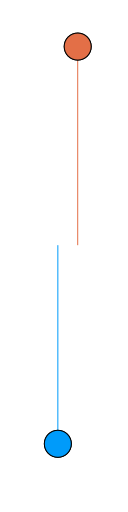
\includegraphics[height=.666\textheight]{pendulum_equilibria}
	\end{minipage}

	\vspace{1cm}
\end{frame}

\begin{frame}[t, c]{The simple pendulum}{Fixed points}
	\centering
	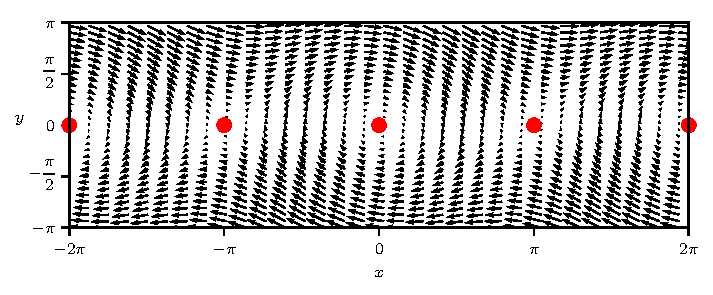
\includegraphics[width=.8\textwidth]{pendulum_fixed_points}
\end{frame}

\begin{frame}[t, c]{The simple pendulum}{Trajectories}
	\centering
	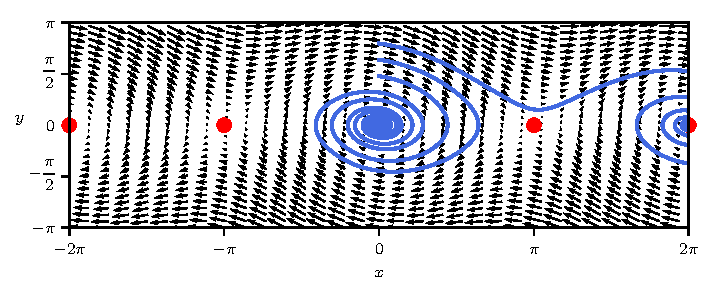
\includegraphics[width=.8\textwidth]{pendulum_fixed_trajectories_bis}
\end{frame}

\begin{frame}[t, c]{The simple pendulum}{Linearizing the system in the downward position}
	\begin{minipage}{.68\textwidth}
		\begin{itemize}
			\item Let us linearize the equations in the vicinity of the downward position.
			The equations of motion become
			%
			\[
				\displaystyle \frac{\mathrm{d}}{\mathrm{d}t} \begin{bmatrix} x \\ y \end{bmatrix} = \underbrace{\begin{bmatrix} 0 & 1 \\ -\omega_0^2 & -2k \end{bmatrix}}_{\bm{A}} \begin{bmatrix} x \\ y \end{bmatrix}.
			\]

			\item In this small oscillation limit, we recover the damped harmonic oscillator model.

			\item For all (positive) values of the friction parameter \(k\), the eigenvalues \( \lambda \) of \( \bm{A} \) are characterized by
			%
			\[
				\Re(\lambda) < 0
			\]
			%
			indicating that this equilibrium position is \alert{\textbf{linearly stable}}.
		\end{itemize}
	\end{minipage}%
	\hfill
	\begin{minipage}{.28\textwidth}
		\centering
		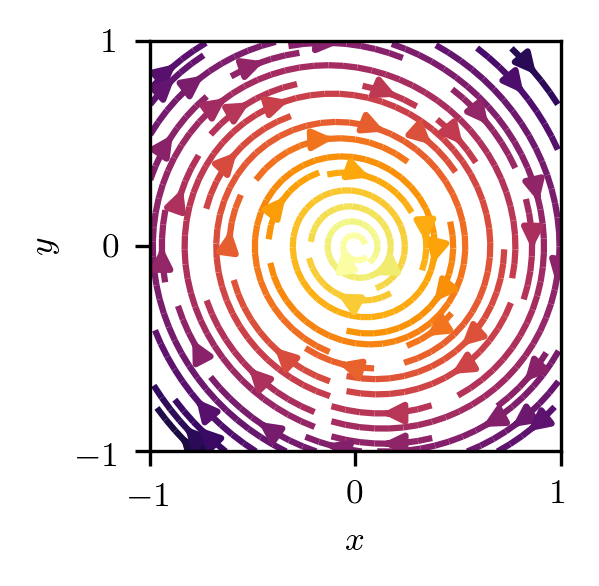
\includegraphics[width=\textwidth]{pendulum_downward_stab}
	\end{minipage}

	\vspace{1cm}
\end{frame}


\begin{frame}[t, c]{The simple pendulum}{Linearizing the system in the upward position}
	\begin{minipage}{.28\textwidth}
		\centering
		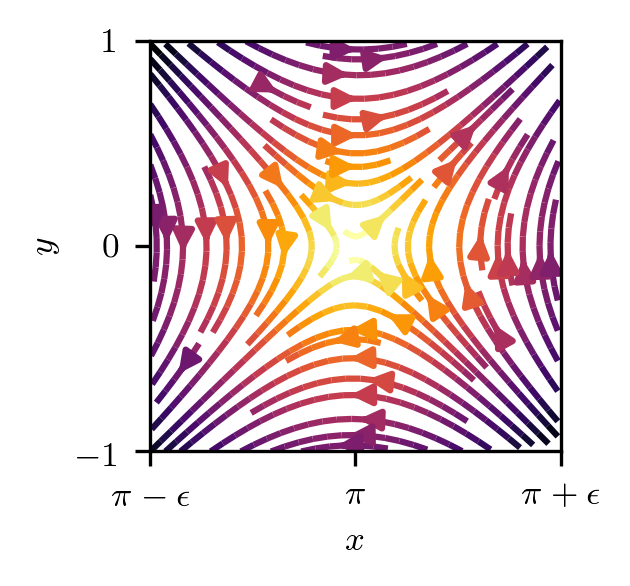
\includegraphics[widht=\textwidth]{pendulum_upward_stab}
	\end{minipage}%
	\hfill
	\begin{minipage}{.68\textwidth}
		\begin{itemize}
			\item Let us linearize the equations in the vicinity of the upward position.
			The equations of motion become
			%
			\[
				\displaystyle \frac{\mathrm{d}}{\mathrm{d}t} \begin{bmatrix} x \\ y \end{bmatrix} = \underbrace{\begin{bmatrix} 0 & 1 \\ -\omega_0^2 & 2k \end{bmatrix}}_{\bm{A}} \begin{bmatrix} x \\ y \end{bmatrix}.
			\]

			\item For all (positive) values of the friction parameter \(k\), the eigenvalues \( \lambda \) of \( \bm{A} \) are characterized by
			%
			\[
				\Re(\lambda) > 0
			\]
			%
			indicating that this equilibrium position is \alert{\textbf{linearly unstable}}.
		\end{itemize}
	\end{minipage}

	\vspace{1cm}
\end{frame}

\begin{frame}[t, c]{The simple pendulum}{Conclusion}
	\begin{minipage}{.68\textwidth}
		\begin{itemize}
			\item The simple pendulum by itself is a fairly boring system.
			\begin{itemize}
				\item[\( \hookrightarrow \)] Two fixed points, one linearly stable and one linearly unstable.
				\item[\( \hookrightarrow \)] For \( t \to \infty \), the system eventually settles in the stable fixed point due to the dissipative nature of the system.
			\end{itemize}

			\bigskip

			\item Its brother, the double pendulum, has far richer dynamics!
			\begin{itemize}
				\item[\( \hookrightarrow \)] Harder to study though because of its four-dimensional phase space.
				\item[\( \hookrightarrow \)] In the Hamiltonian limit (i.e.\ no friction), special numerical techniques need to be used to verify the physics.
			\end{itemize}
		\end{itemize}
	\end{minipage}%
	\hfill
	\begin{minipage}{.28\textwidth}
		\centering
		\movie[width=\textwidth, autostart, loop]{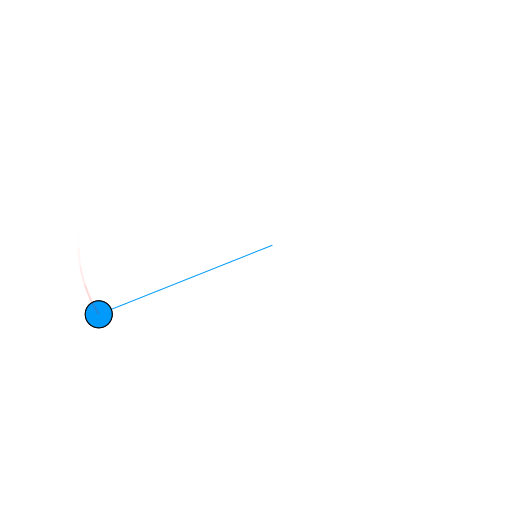
\includegraphics[width=\textwidth]{pendulum_image}}{imgs/single_pendulum.mp4}
	\end{minipage}

	\vspace{1cm}
\end{frame}

\begin{frame}[t, c]{}{}
	\centering

	{\Large \textbf{Case study II}}

	\bigskip

	\textgre{\textbf{The Lorenz system}}

	\vspace{-2cm}
\end{frame}

\begin{frame}[t, c]{The Lorenz system}{A simplified model of atmospheric convection}
	\begin{minipage}{.58\textwidth}
		\begin{itemize}
			\item It is a (very) simplified model of atmospheric convection which can be derived analytically from the Navier-Stokes equations.

			\bigskip

			\item In its most common form, it reads
			%
			\[
				\begin{aligned}
					& \dot{x} = \sigma ( y - x ) \\
					& \dot{y} = x (\rho - z) - y \\
					& \dot{z} = xy - \beta z.
				\end{aligned}
			\]

			\medskip

			\item In what follows, we set \( \sigma = 10 \) and \( \beta = \nicefrac{8}{3} \) and study the evolution of the system as \( \rho \) varies.
		\end{itemize}
	\end{minipage}%
	\hfill
	\begin{minipage}{.38\textwidth}
		\centering
		\movie[width=\textwidth, autostart, loop]{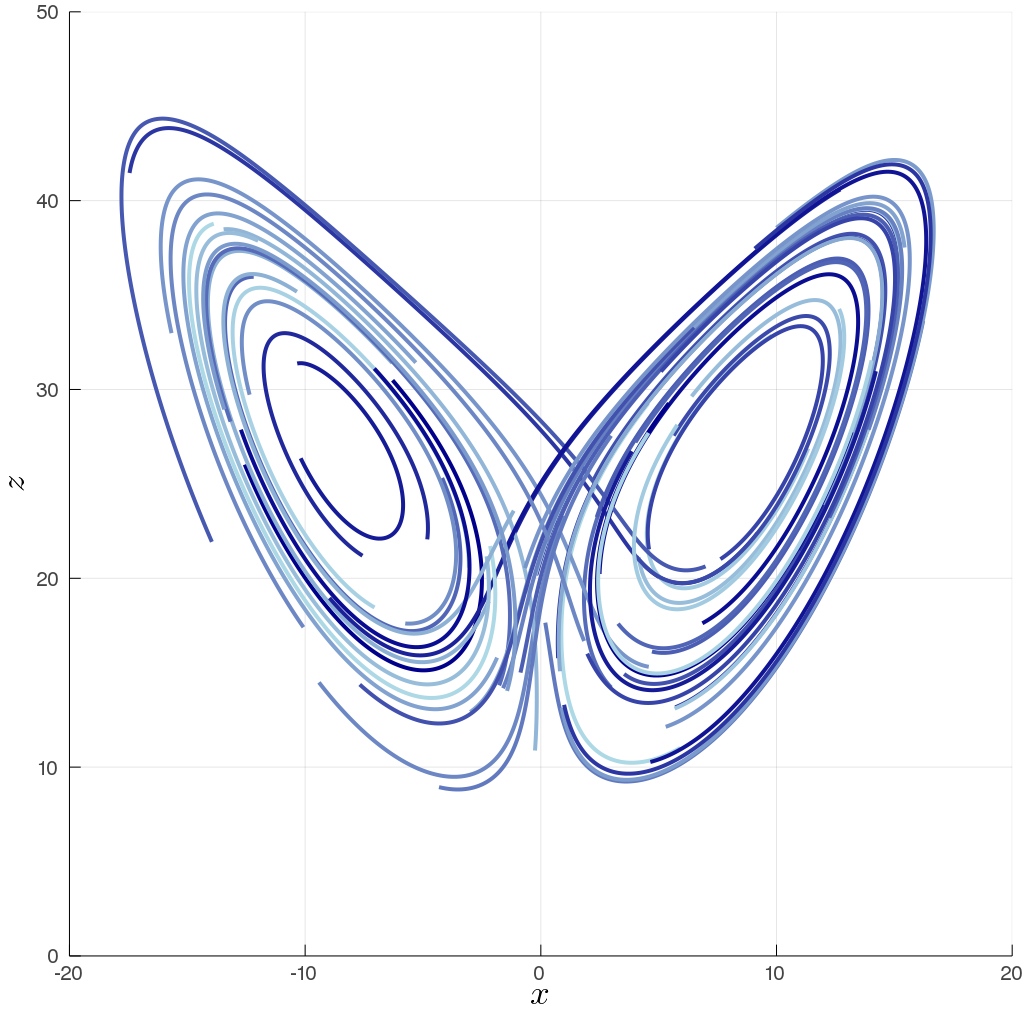
\includegraphics[width=\textwidth]{Lorenz_video_image}}{imgs/lorenz_system.mp4}
	\end{minipage}

	\vspace{1cm}
\end{frame}

\begin{frame}[t, c]{The Lorenz system}{A (popular) chaotic system}
	\begin{minipage}{.38\textwidth}
		\centering
		\movie[width=\textwidth, autostart, loop]{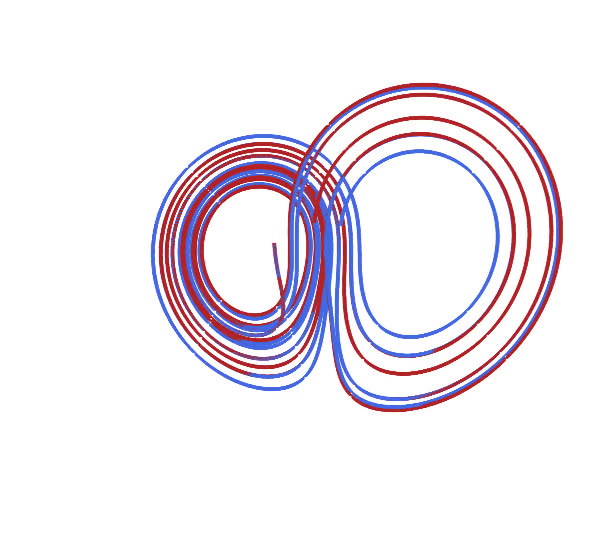
\includegraphics[width=\textwidth]{image_video_lorenz}}{imgs/Lorenz_attractor_JC.mp4}
	\end{minipage}%
	\hfill
	\begin{minipage}{.58\textwidth}
		\begin{itemize}
			\item For certain range of parameters, the Lorenz system exhibits chaotic dynamics.

			\medskip

			\item The corresponding \emph{attractor} is known as a \emph{strange attractor}.
			\begin{itemize}
				\item[\( \hookrightarrow \)] It cannot be described by standard geometry.
				\item[\( \hookrightarrow \)] One instead needs to use \emph{fractal geometry} (its dimension is 2.06 for instance).
			\end{itemize}

			\medskip

			\item Its double-winged structure is one of the reason why the sensitivity to initial condition is called the \emph{butterfly effect} in mainstream media.
		\end{itemize}
	\end{minipage}

	\vspace{1cm}
\end{frame}

\begin{frame}[t, c]{}{}
	\centering

	{\Large \textbf{Case study III}}

	\bigskip

	\textgre{\textbf{The logistic map}}

	\vspace{-2cm}
\end{frame}

\begin{frame}[t, c]{The logistic map}{A discrete-time nonlinear system}
	\begin{minipage}{.28\textwidth}
		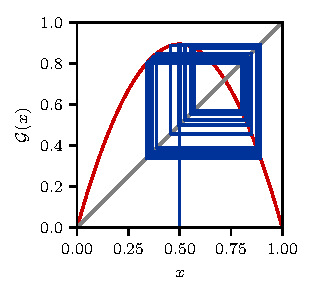
\includegraphics[width=\textwidth]{logistic_map_cobweb_plot_8}
	\end{minipage}%
	\hfill
	\begin{minipage}{.68\textwidth}
		\begin{itemize}
			\item Very simple model for population dynamics popularized during the 1970's by Robert May.
			\begin{itemize}
				\item[\( \hookrightarrow \)] Played a crucial role in the development of chaos theory.
			\end{itemize}

			\medskip

			\item The model reads
			%
			\[
				x_{k+1} = \mu x_k ( 1 - x_k ).
			\]

			\item Despite its simplicity, the system can exhibit complex dynamics.
			\begin{itemize}
				\item[\( \hookrightarrow \)] Fixed points, periodic orbits, chaotic dynamics.
			\end{itemize}

			\medskip

			\item You are strongly encourage to implement this model yourself and play with it!
			\begin{itemize}
				\item [\( \hookrightarrow \)] Only a handful lines of code are needed.
			\end{itemize}

		\end{itemize}
	\end{minipage}

	\vspace{1cm}
\end{frame}

\begin{frame}[t, c]{The logistic map}{Bifurcation diagram}
	\centering
	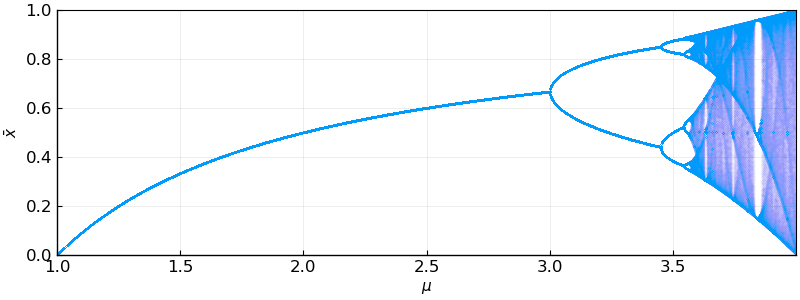
\includegraphics[width=.8\textwidth]{logistic_map_bifucartion_diagram_1}
\end{frame}

\begin{frame}[t, c]{The logistic map}{Bifurcation diagram}
	\centering
	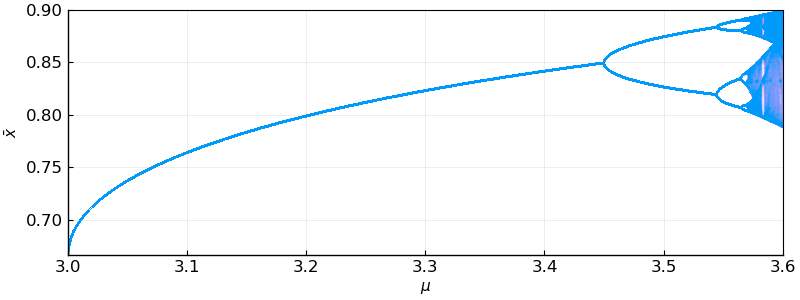
\includegraphics[width=.8\textwidth]{logistic_map_bifucartion_diagram_2}
\end{frame}

\begin{frame}[t, c]{The logistic map}{Bifurcation diagram}
	\centering
	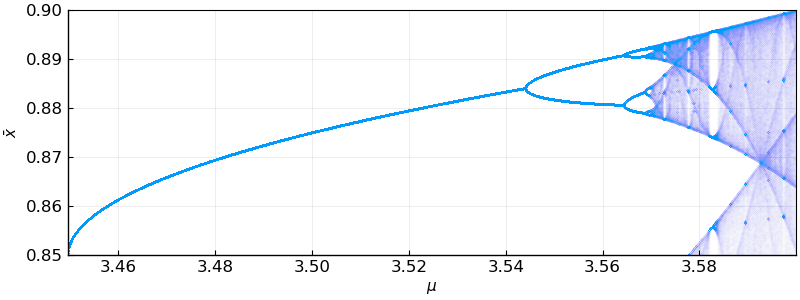
\includegraphics[width=.8\textwidth]{logistic_map_bifucartion_diagram_3}
\end{frame}

\begin{frame}[t, c]{The logistic map}{Connection with the Mandelbrot set}
	\begin{minipage}{.58\textwidth}
		\begin{itemize}
			\item The logistic map is closely related to the Mandelbrot set, a famous fractal object.

			\medskip

			\item Given the map \( z_{k+1} = z_k^2 + c \) with \( c \in \mathbb{C} \), the Mandelbrot set is defined as
			%
			\[
				c \in \mathcal{M} \iff \lim_{k \to \infty} \vert z_{k+1} \vert \leq 2.
			\]

			\medskip

			\item The last course of this class will be dedicated to a quick introduction to fractal geometry.
		\end{itemize}
	\end{minipage}%
	\hfill
	\begin{minipage}{.38\textwidth}
		\centering
		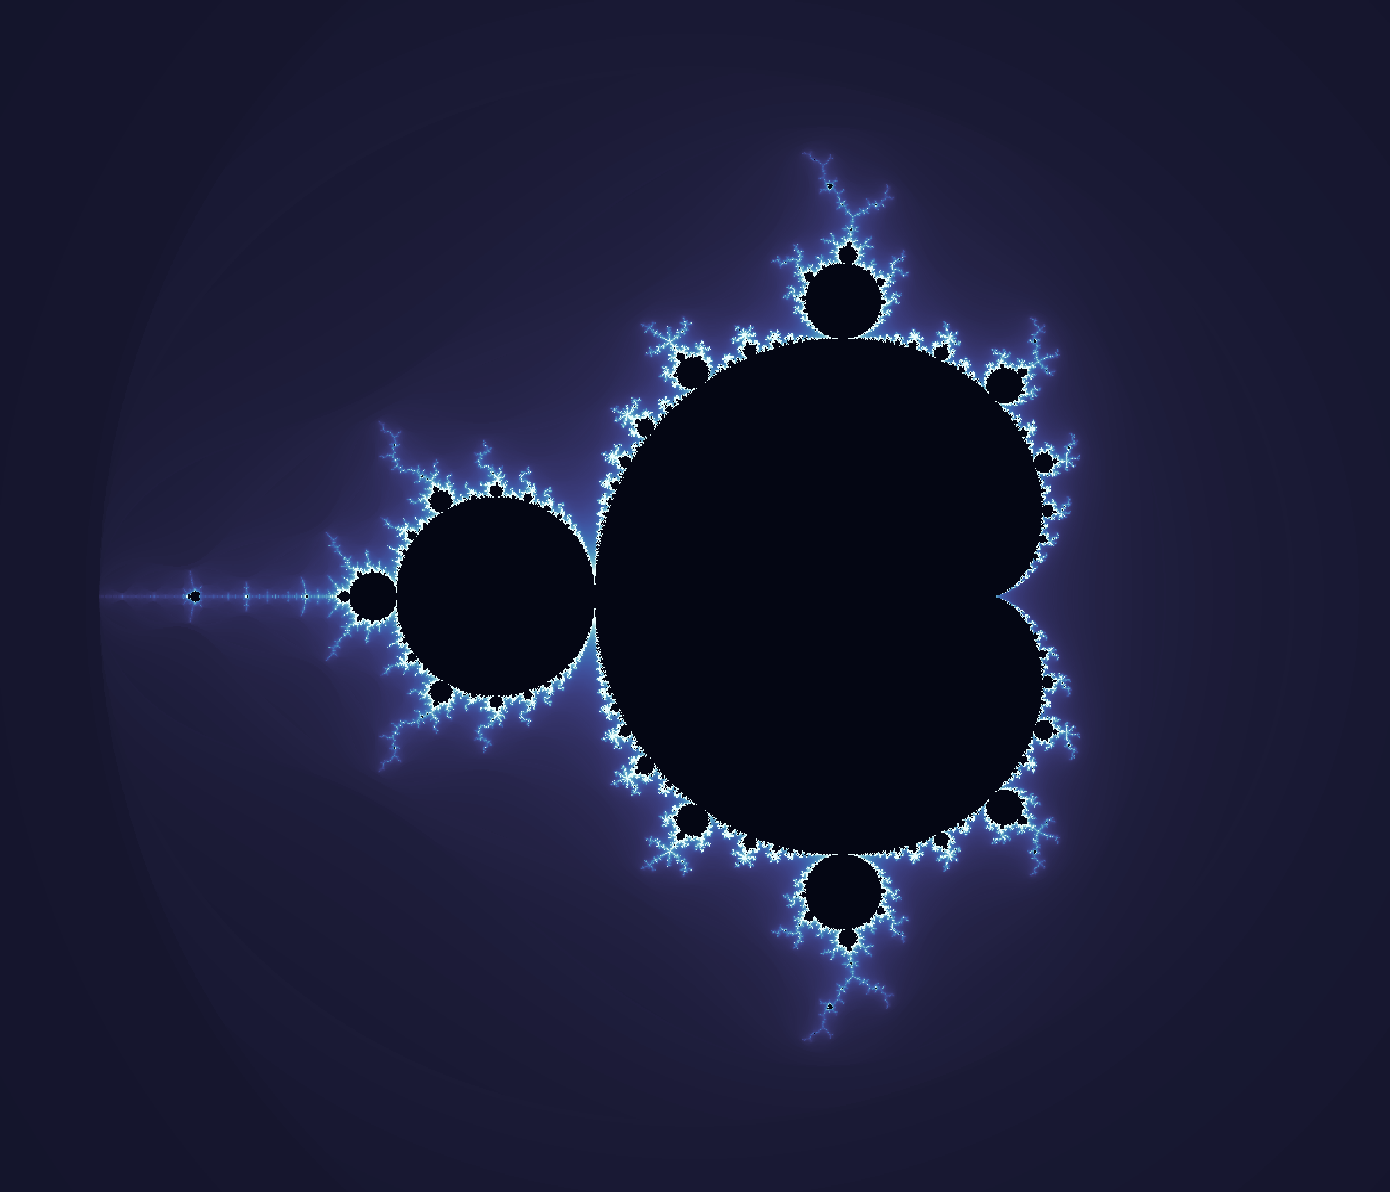
\includegraphics[width=\textwidth]{Mandelbrot_set}
	\end{minipage}

	\vspace{1cm}
\end{frame}

\end{document}
